\newpage
\begin{figure*}[t]
\centering
		\begin{subfigure}[b]{0.3\textwidth}
                 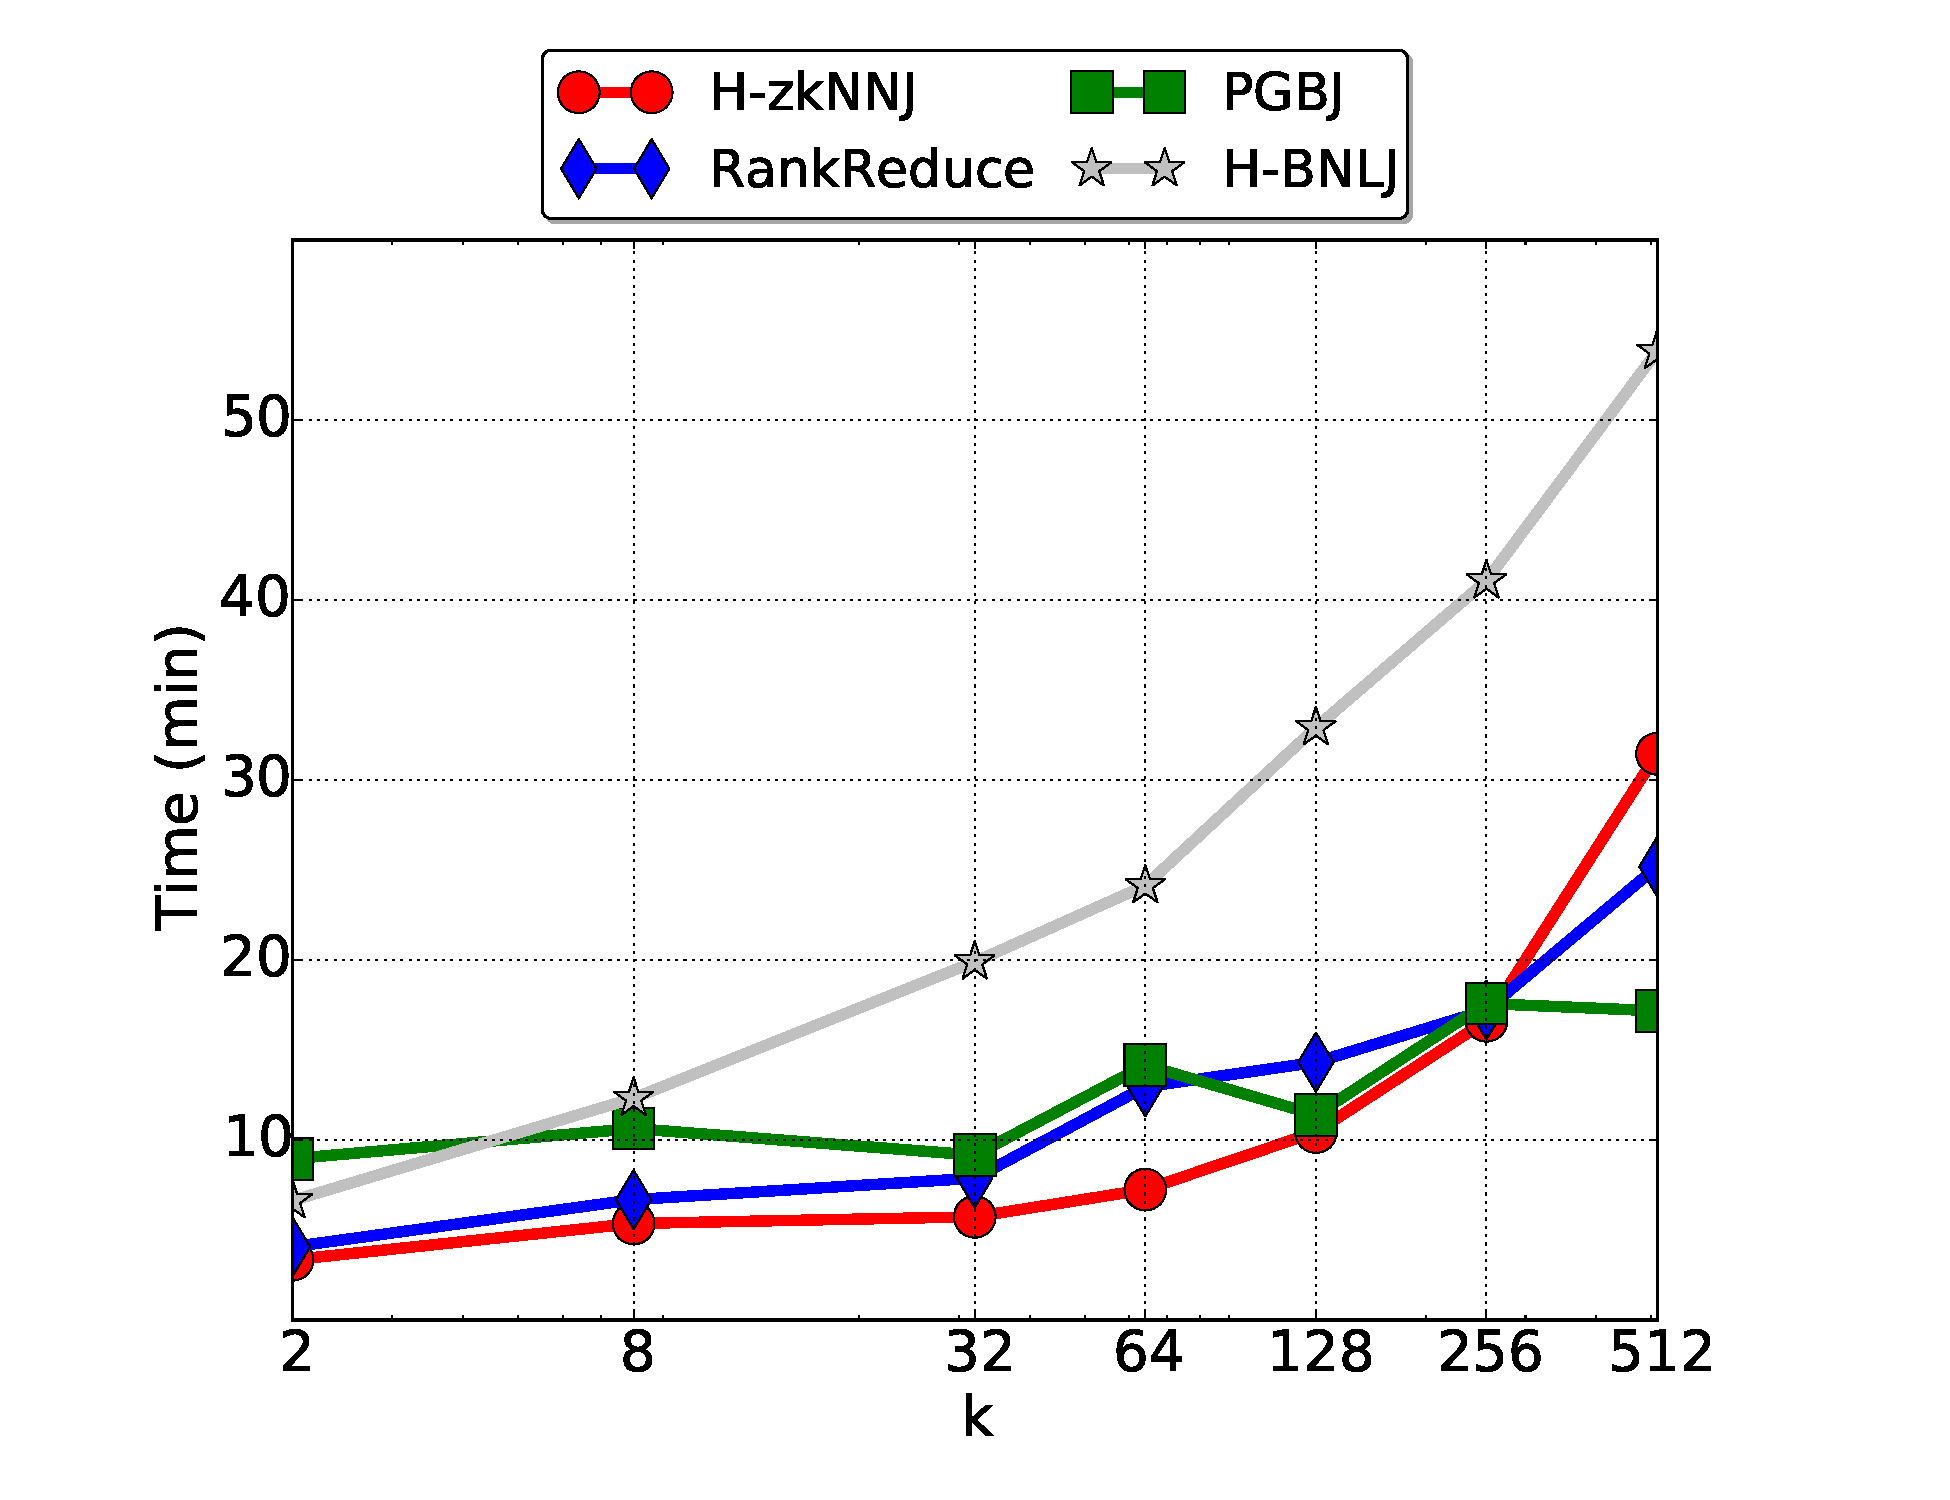
\includegraphics[width=\textwidth]{img-perf/geo/k/time.pdf} 
                \caption{Time\label{fig:geo_k_time}} 
                
        \end{subfigure}%
        \begin{subfigure}[b]{0.3\textwidth}
                 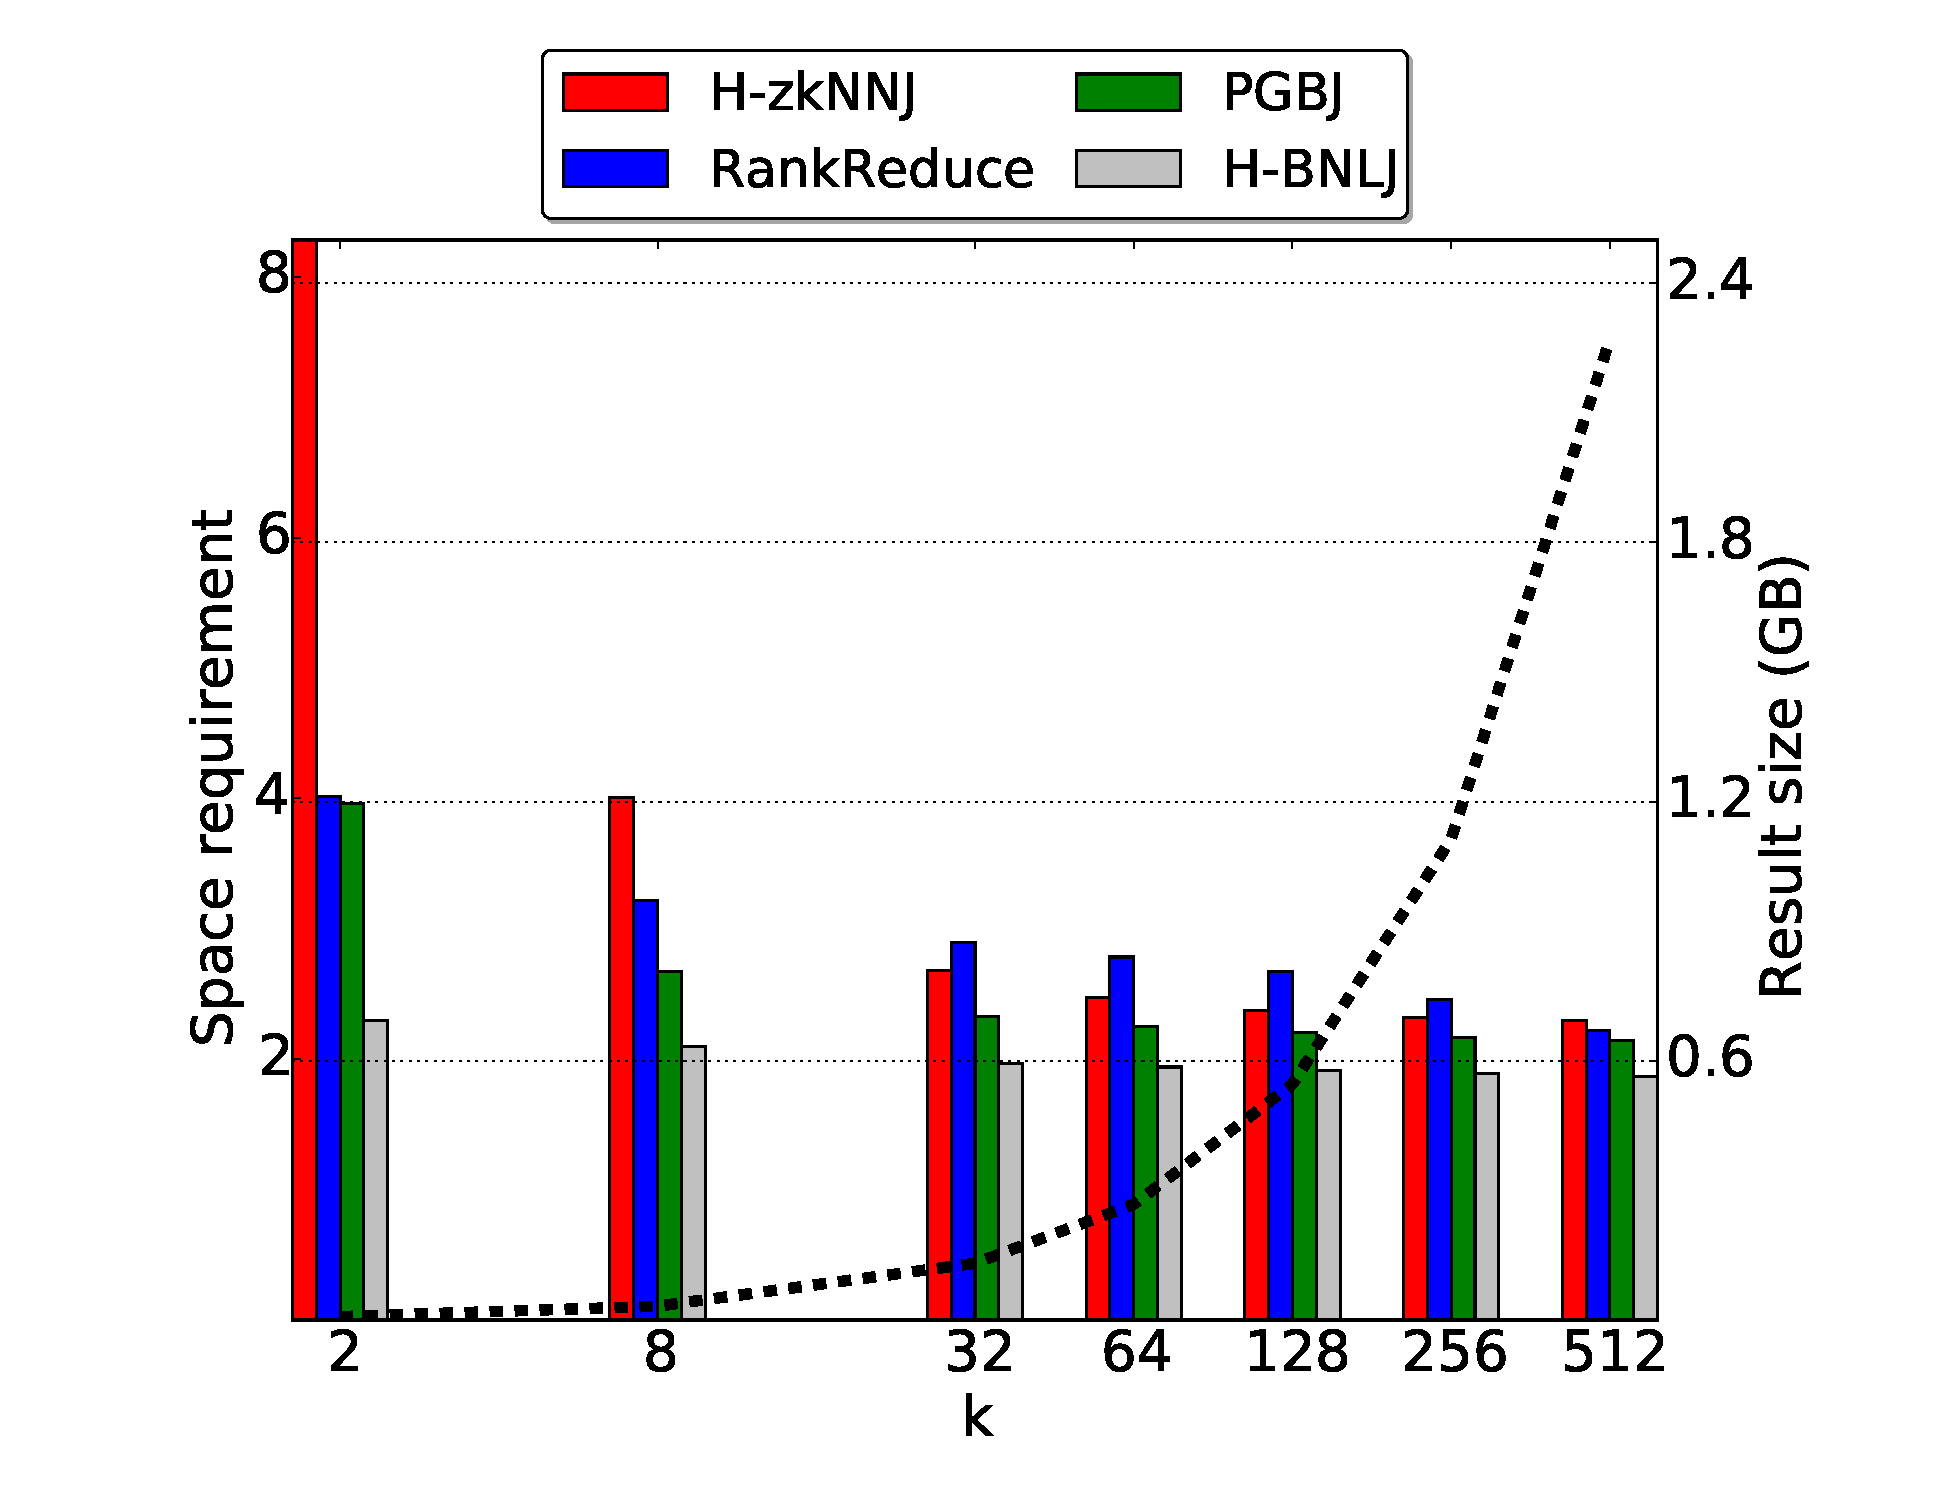
\includegraphics[width=\textwidth]{img-perf/geo/k/memory.pdf} 
                \caption{Result size and Disk Usage\label{fig:geo_k_memory} \TODO{Why does disk usage of H-zkNNJ decreases so much w 2}}
                
        \end{subfigure}%
        \begin{subfigure}[b]{0.3\textwidth}
                 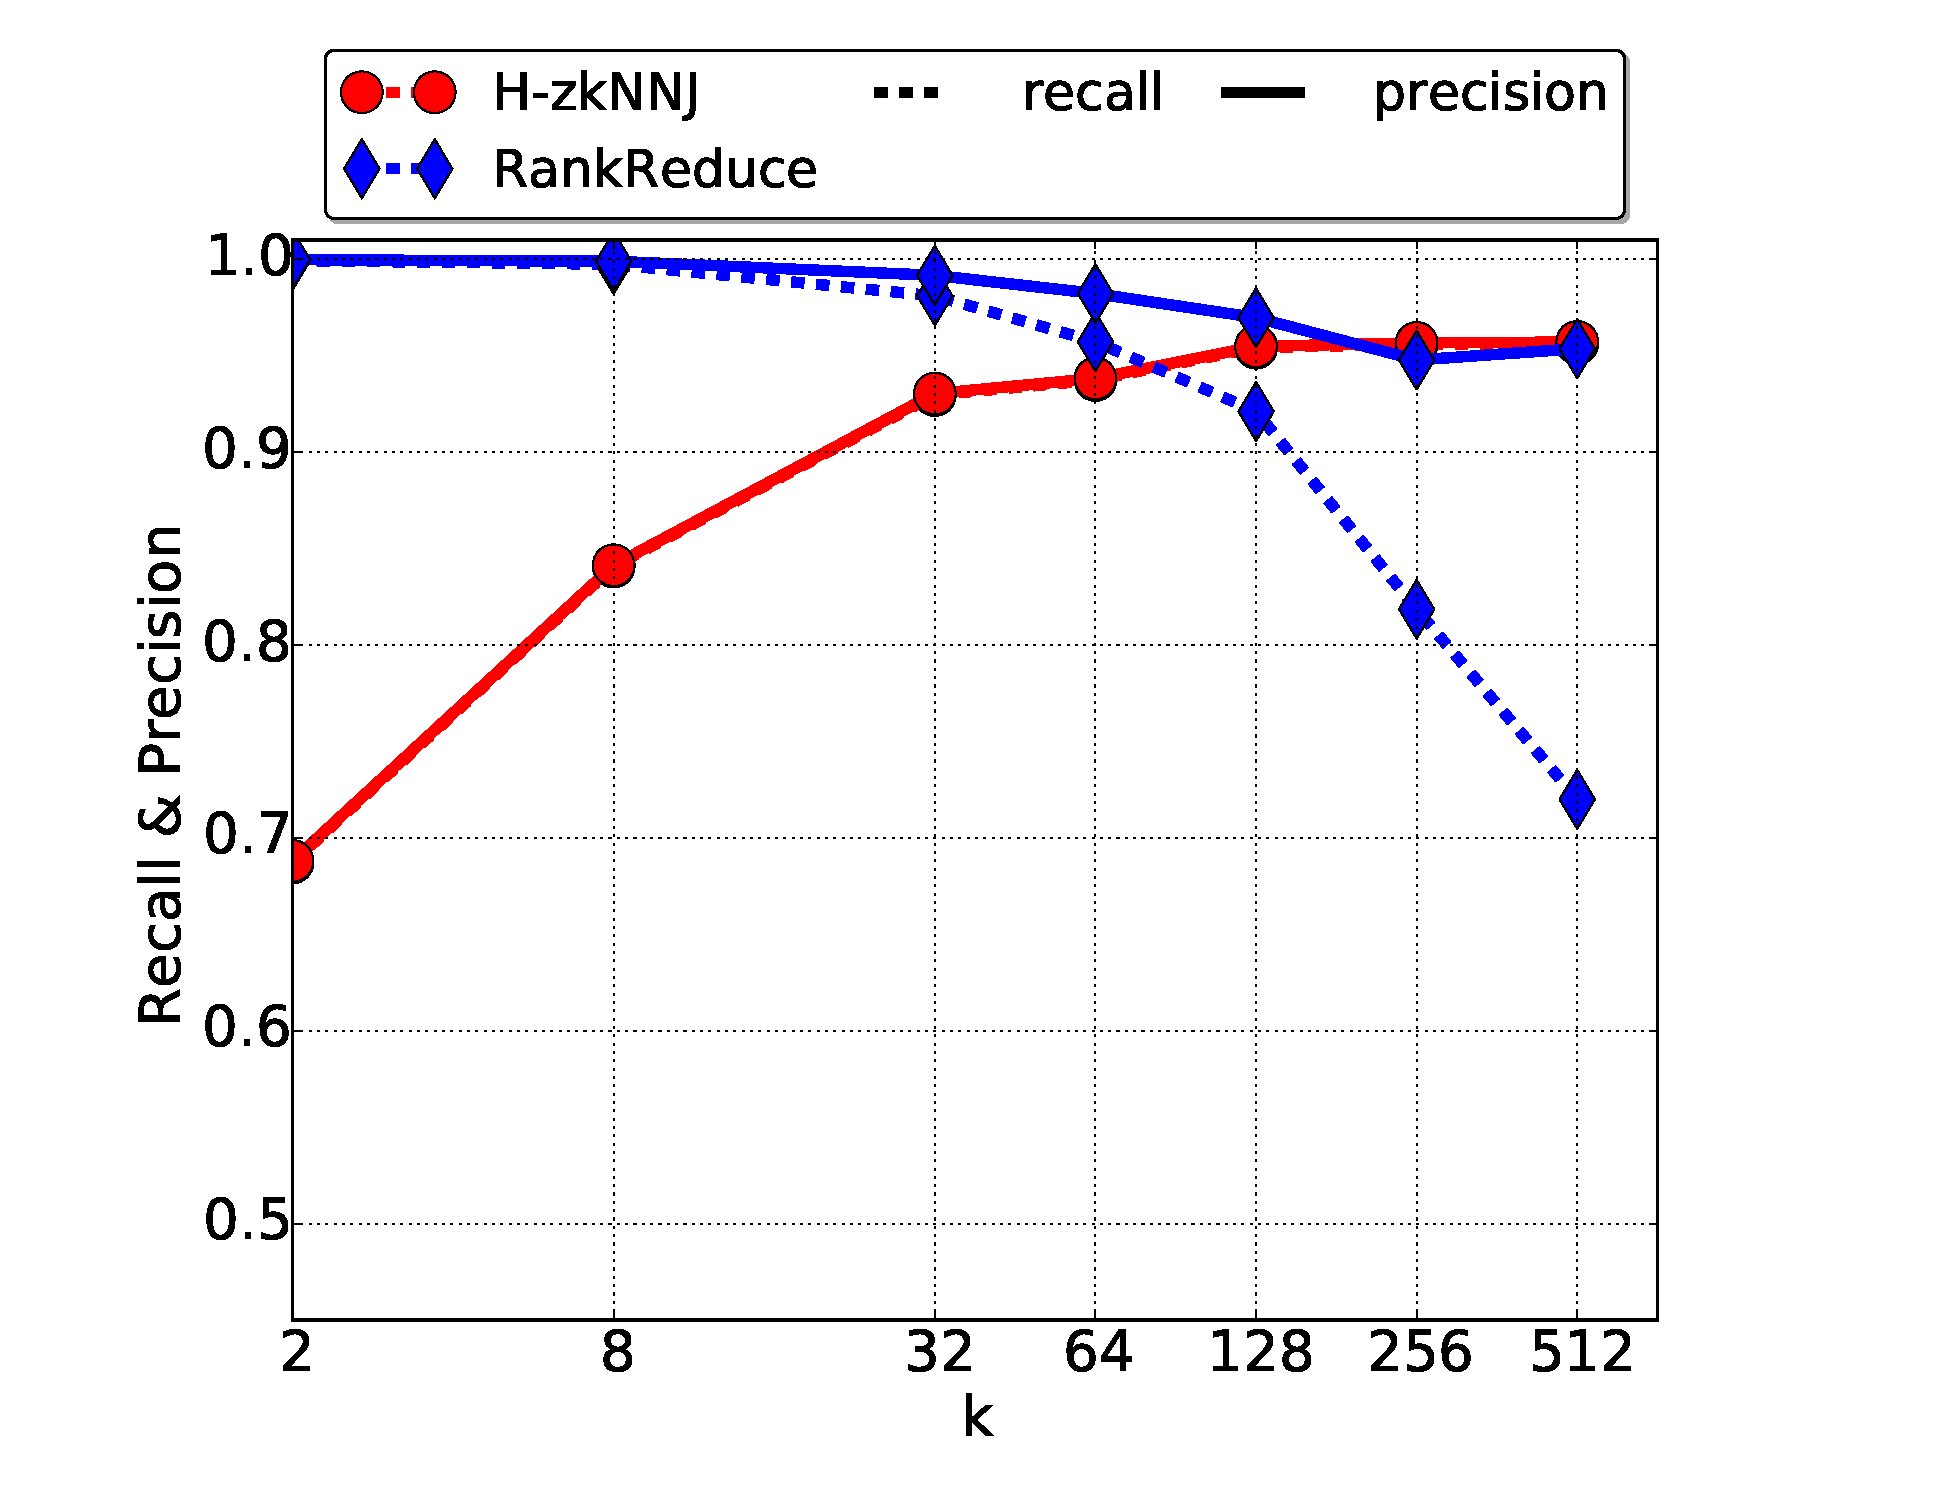
\includegraphics[width=\textwidth]{img-perf/geo/k/accuracy.pdf} 
                \caption{Accuracy\label{fig:geo_k_acc}}
                
        \end{subfigure}%
 \caption{Geo dataset with 200k records (50k for H-BNLJ) , impact of $K$ }\label{fig:geo_impact_k}
%\TODOREP{
%EXPLICATION STORAGE HZKNN
%pour comprendre le ratio de storage de zvalue il faut comprendre les etapes des job\\
%\\
%ROUND 1 : creer les copies de tous les records + partioner R et S\\
%ROUND 2 : candidats de chaque partition\\
%ROUND 3 : vrai KNN\\
%\\
%Qu'est ce qui change lorsqu on change K ?\\
%\\
%ROUND 1 non , meme partout\\
%ROUND 2 : oui on prend plus de K\\
%ROUND 3 :  oui on prend plus de K\\
%\\
%=> ROUND 2 est proportionel à ROUND 3\\
%Ainsi qd ROUND 1  le nombre de copie s'approche de nombre de K voulu\\
%alors ca vaut le coup \\
%\\
%example : j'ai 20 data par fichier 3 copie : 60*2 copies en tout\\
%je veux 2 voisins\\
%\\
%round1 : 120 copies creer\\
%round 2 : 20*2*3 = 20 data 2 oisins chacun pour 3 copies = 120\\
%round 3 : 20*2 = 40\\
%\\
%ratio si non compresse serait 240/40 +1 = 7\\
%\\
%je veux 4 voisins\\
%\\
%round1 : 120 copies creer\\
%round 2 : 20*4*3 = 20 data 4 voisins chacun pour 3 copies = 240\\
%round 3 : 20*4 = 80\\
%ratio si non compresse serait 240/80 +1 = 4\\
%\\
%je veux 8 voisins\\
%\\
%round1 : 120 copies creer\\
%round 2 : 20*8*3 = 20 data 8 voisins chacun pour 3 copies = 480\\
%round 3 : 20*8 = 160\\
%ratio si nno compresse serait 480/160 +1 = 4\\
%\\
%9 voisins\\
%\\
%round1 : 120 copies creer\\
%round 2 : 20*9*3 = 20 data 8 voisins chacun pour 3 copies = 540\\
%round 3 : 20*9 = 180\\
%ratio si nno compresse serait 480/160 +1 = 4\\
%\\
%ET HOP CONVERGENCE !
%}
\end{figure*}

%%%%%%%%%%%%%%%%%%%%%%%%%%%%%%%%%%%%%%%%%
%DATA




\begin{figure*}[h]
\centering
		\begin{subfigure}[b]{0.3\textwidth}
                 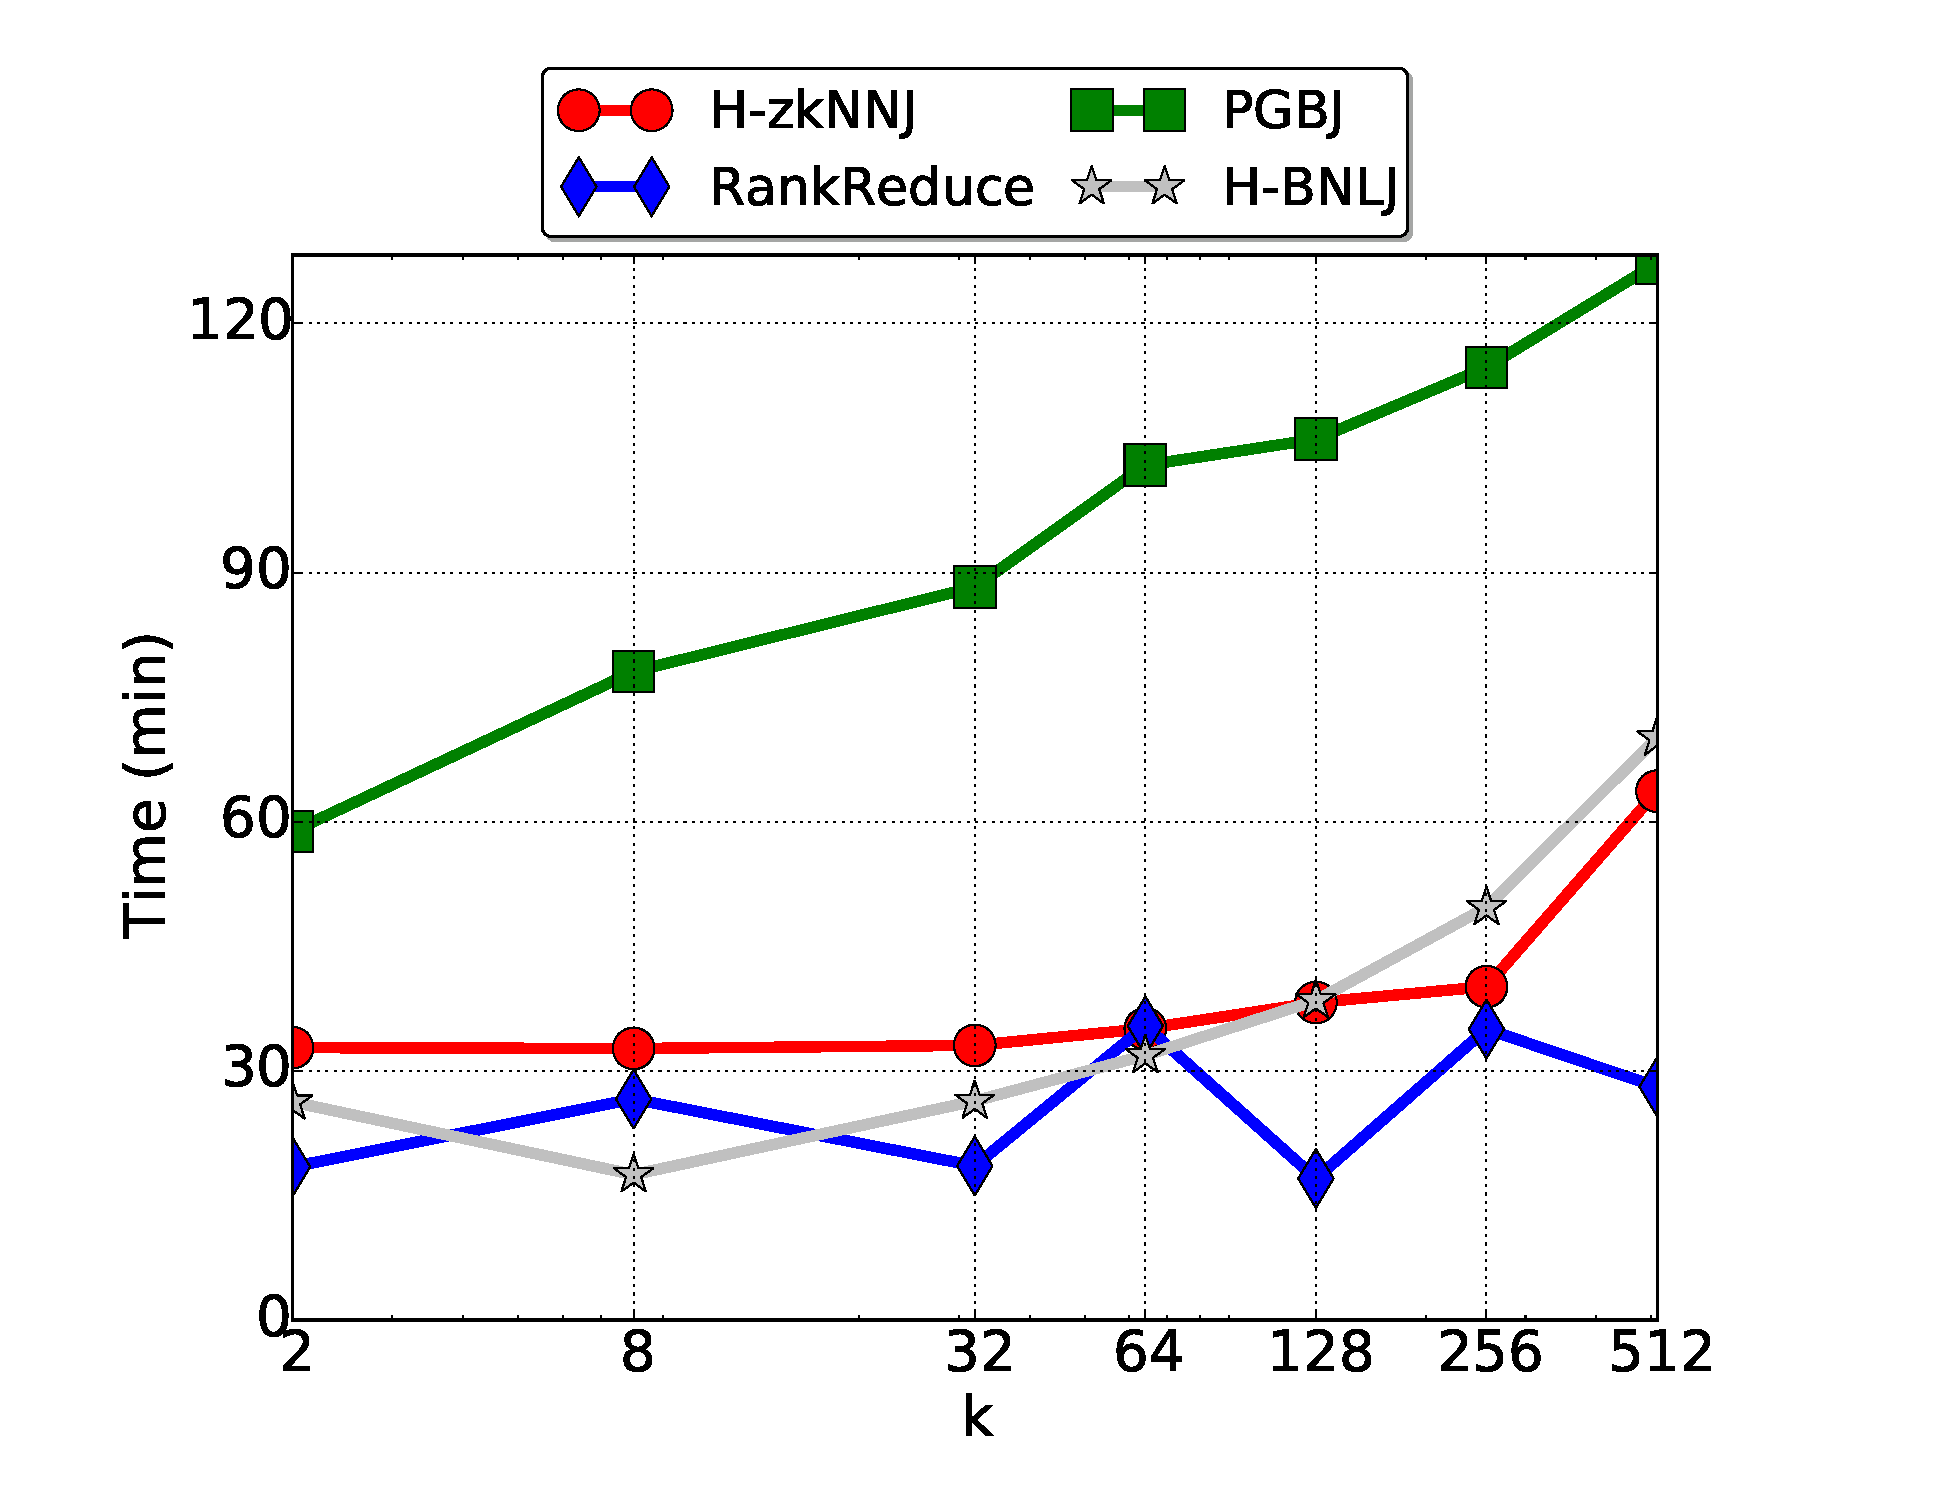
\includegraphics[width=\textwidth]{img-perf/surf/k/time.pdf} 
                \caption{Time\label{fig:surf_k_time} }
                
        \end{subfigure}%
        \begin{subfigure}[b]{0.3\textwidth}
                 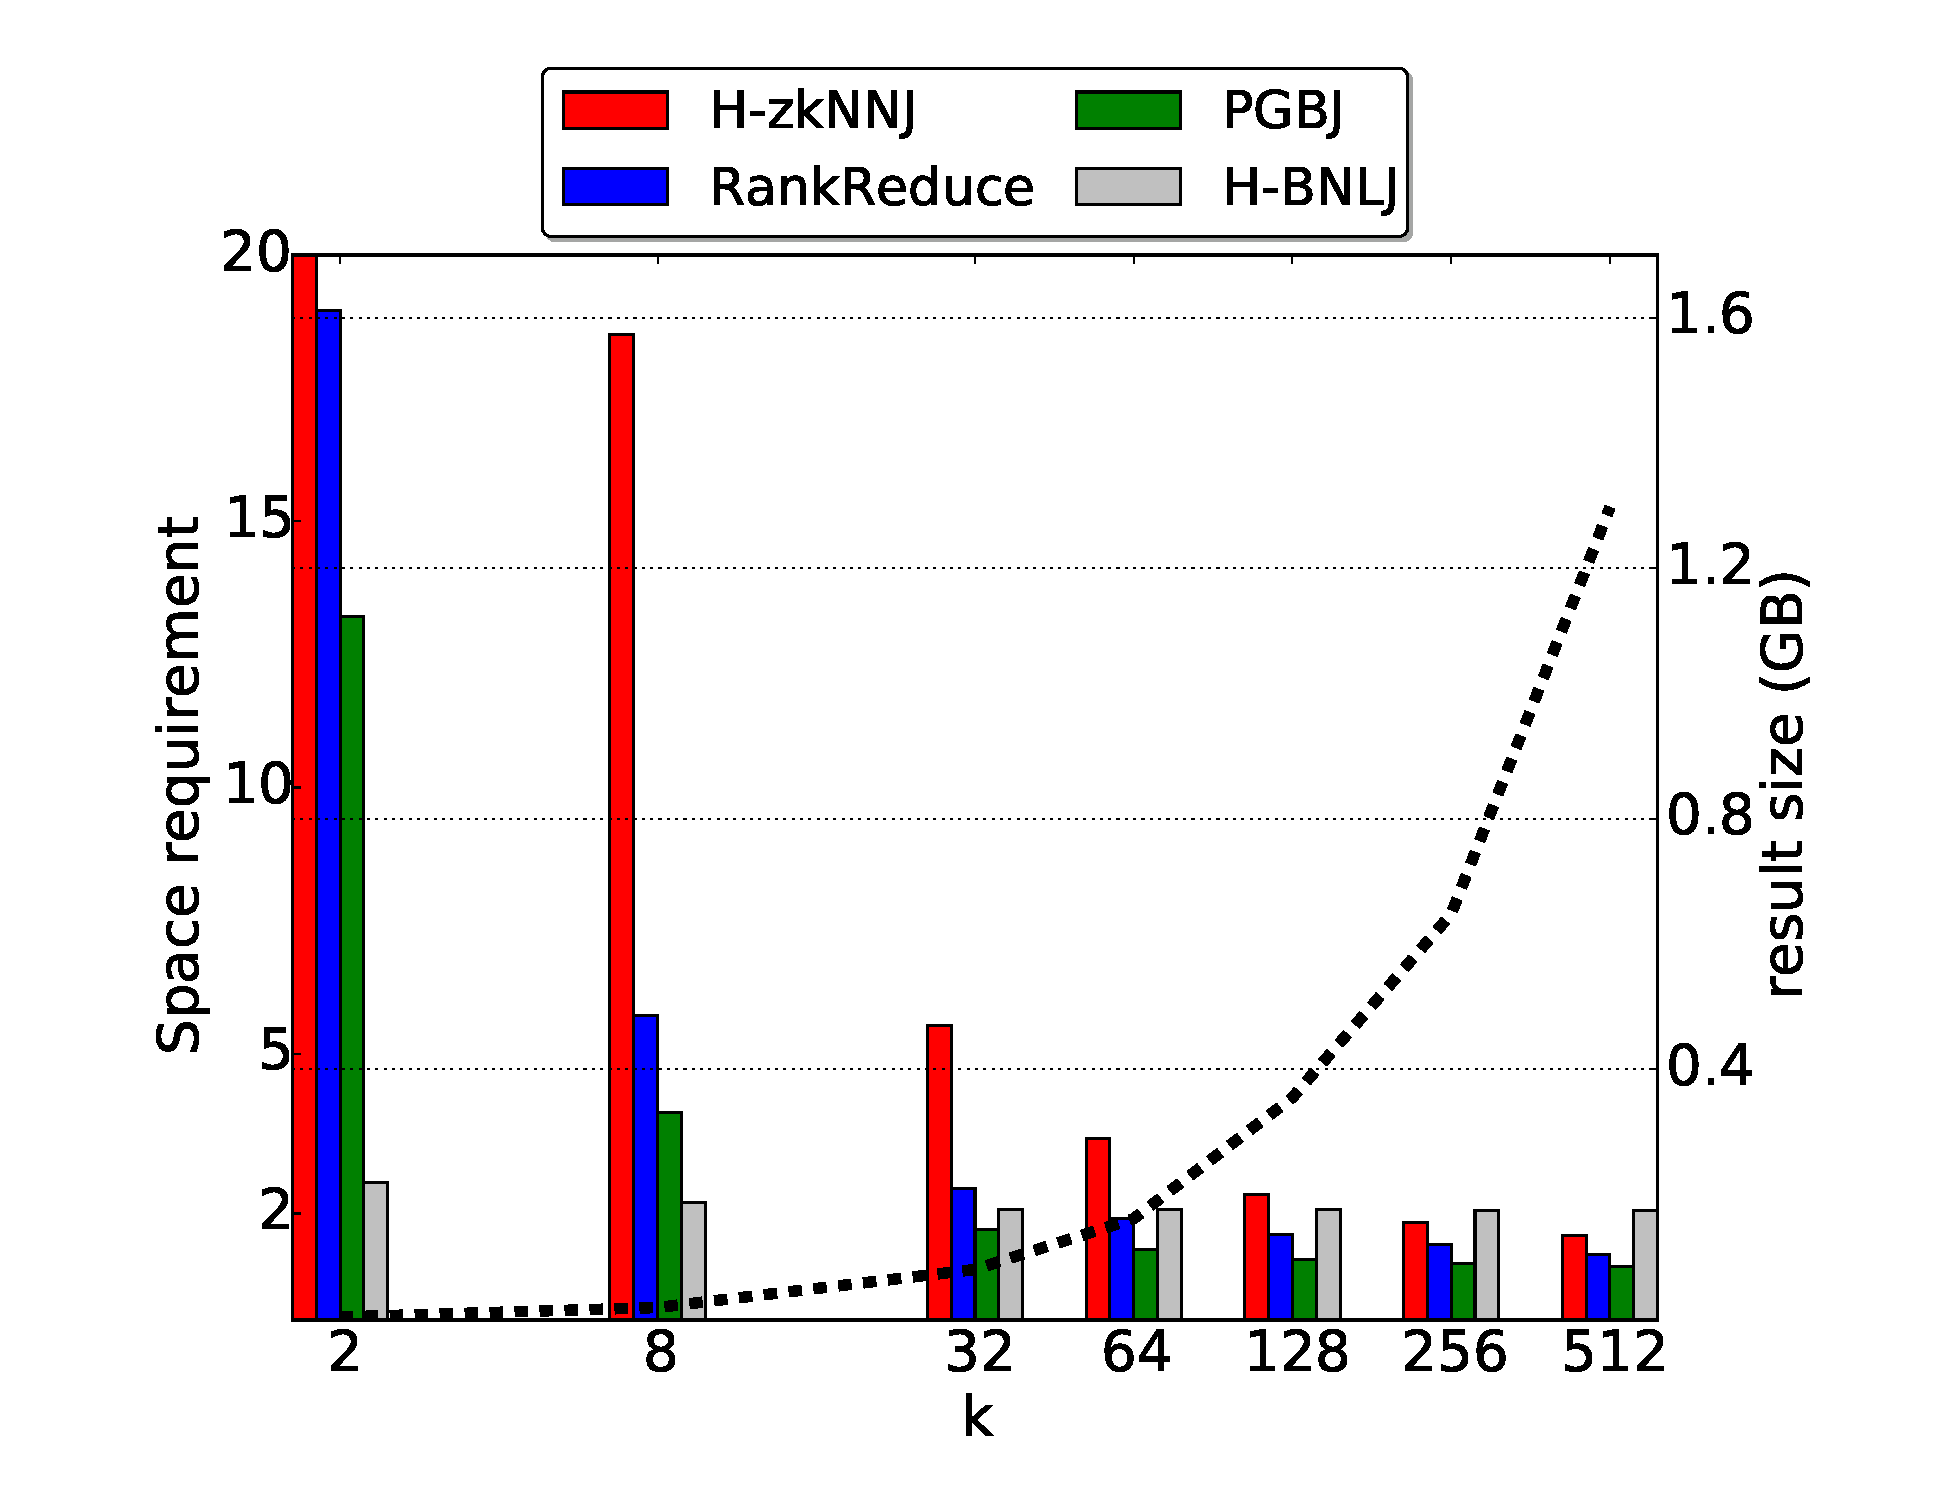
\includegraphics[width=\textwidth]{img-perf/surf/k/memory.pdf} 
                \caption{Result size and Disk Usage\label{fig:surf_k_memory}}
                
        \end{subfigure}%
        \begin{subfigure}[b]{0.3\textwidth}
                 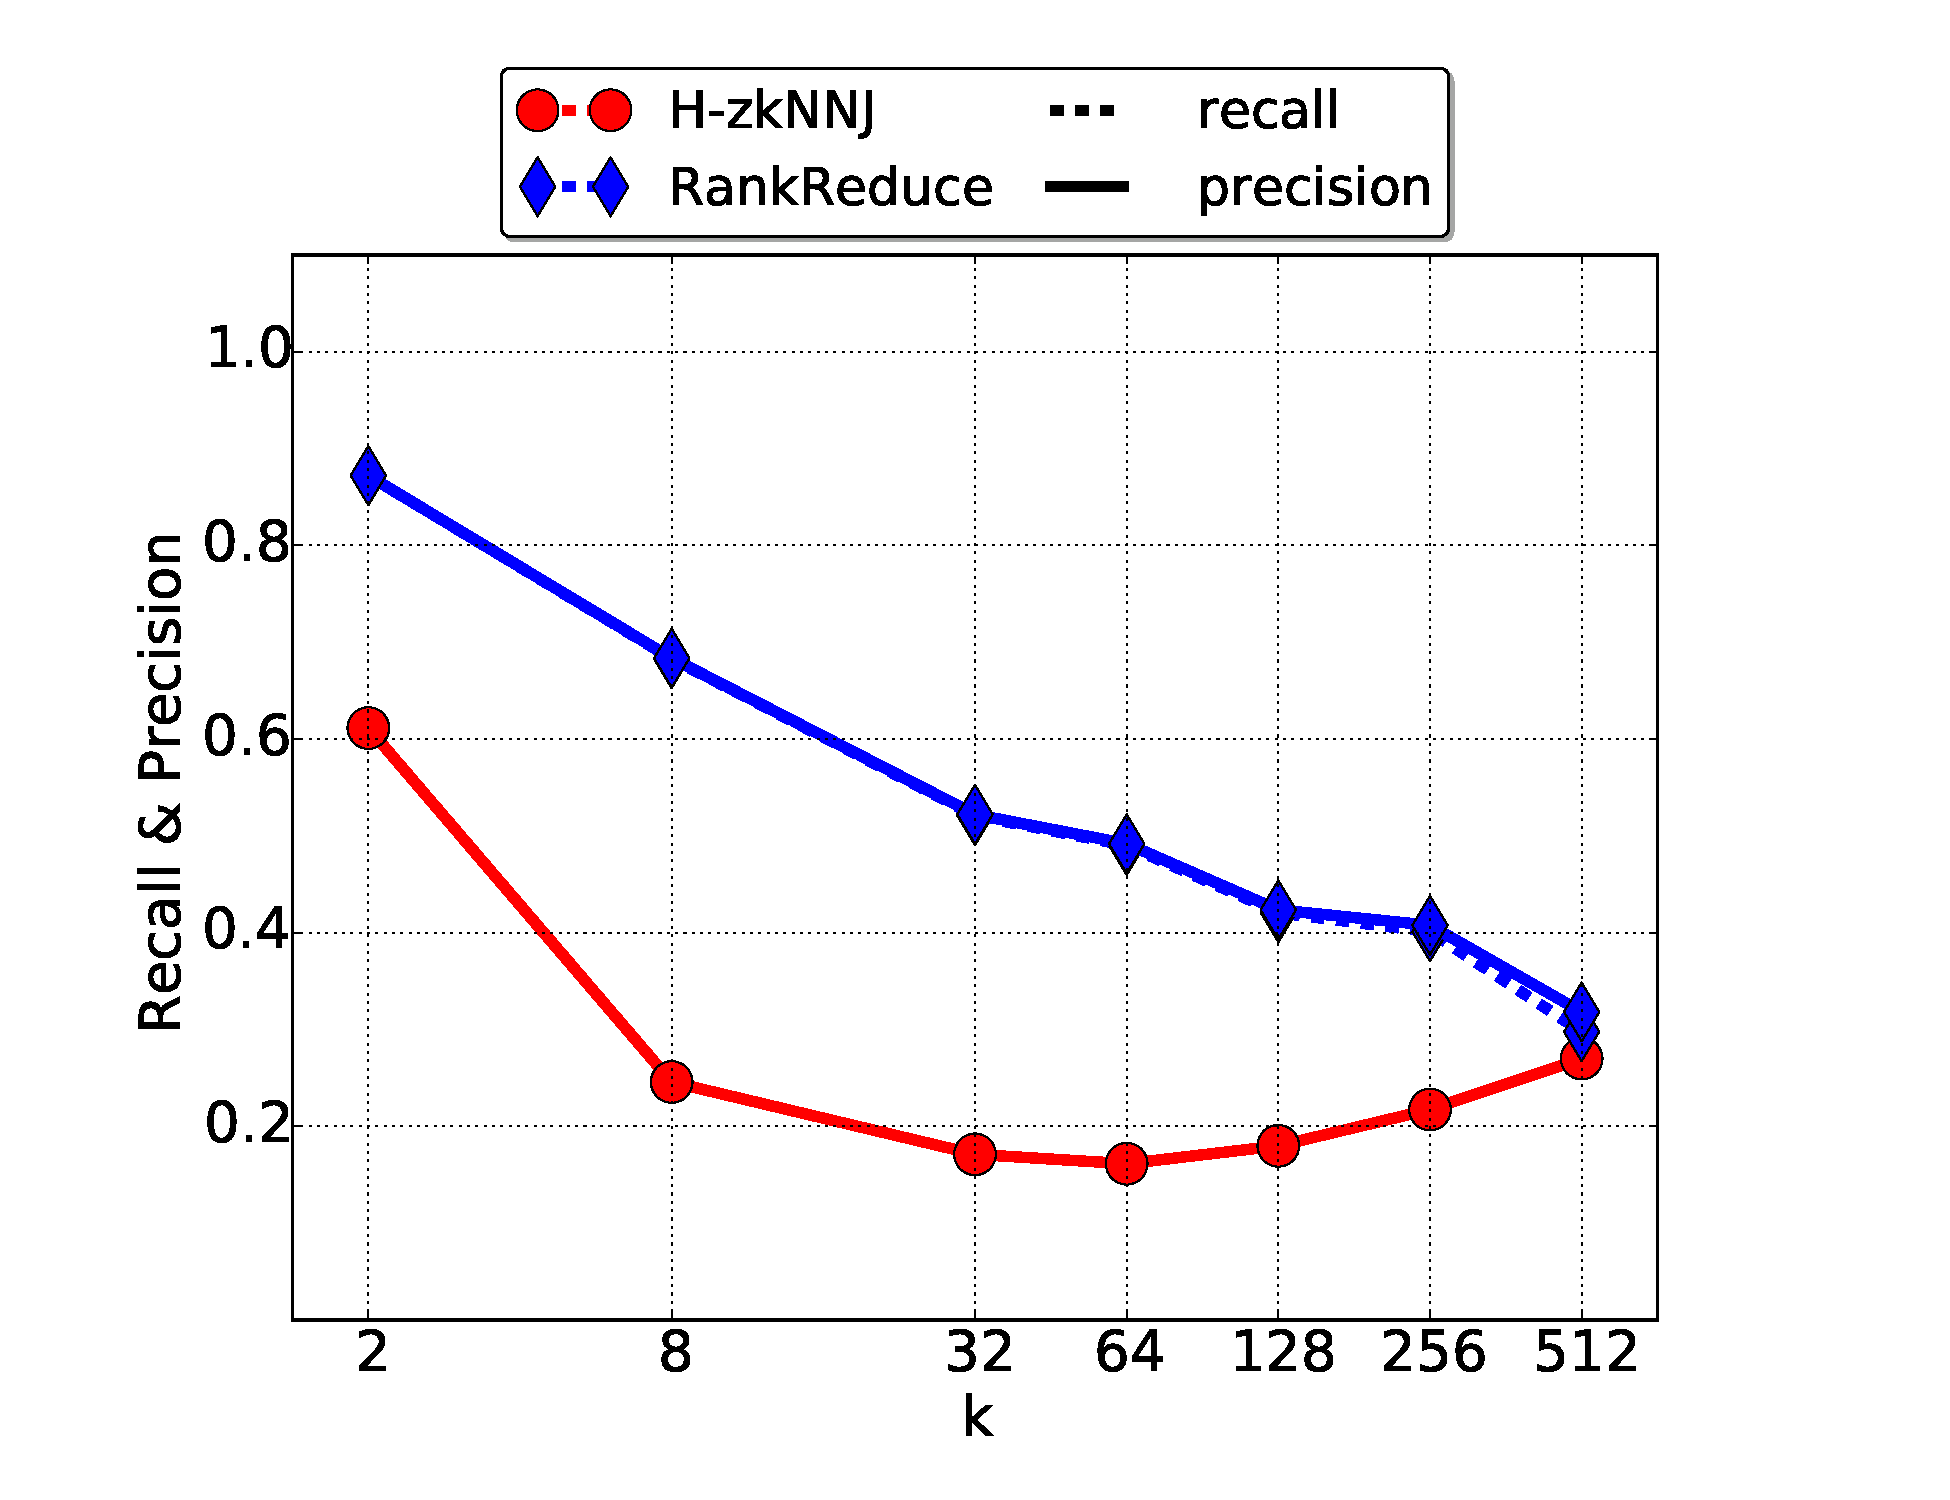
\includegraphics[width=\textwidth]{img-perf/surf/k/accuracy.pdf} 
                \caption{Accuracy\label{fig:surf_k_acc}}
                
        \end{subfigure}%
 \caption{Surf dataset with 50k records, impact of $K$,
%\\ \small{Parameters : \textbf{HBNLJ} : 10partition, \textbf{PGBJ}:$3*10^3 pivots$, Geo grouping, kmeans sample,\textbf{RankReduce}: $L=5,M=7,W=10^7$ HZKNNJ : $3shift$}  
  \label{fig:surf_impact_k}}
%\TODOREP{ Pourr LSH,
%J'ai refait 3 fois les perfs : 
%J'ai ces resultats en dents de scies à chaque fois.
%J'ai regarde les buckets leur nombre aussi en dents de pics...
%c'est du à la phase init avec la hash je fais 5 copies et on est en dimension 128
%la probabilité que les mm données tombent aléatoirement au meme endroit à chaque fois est trop faible lors de la 1ere phase d ou ce phenomene aleatoire ou on a une variation du nombre de buckets qui n'est pas tres signifient mais qui au niveau temps a beaucoup d'impact} 
% J'ai mis fig =figure( figsize=(12, HEIGHT), dpi=80) avec HEIGHT=6 au lieu 8
% pour montrer qu on peut peut etre diminuer la taille des courbes ? NON ?
% }}
\end{figure*}



%%%%%%%%%%%%%%%%%%%%%%%%%%%%%%%%%%%%%%%%%%%%
%LOAD BALANCING
%
%\begin{figure*}[h]
%\centering
%		\begin{subfigure}[b]{0.3\textwidth}
%                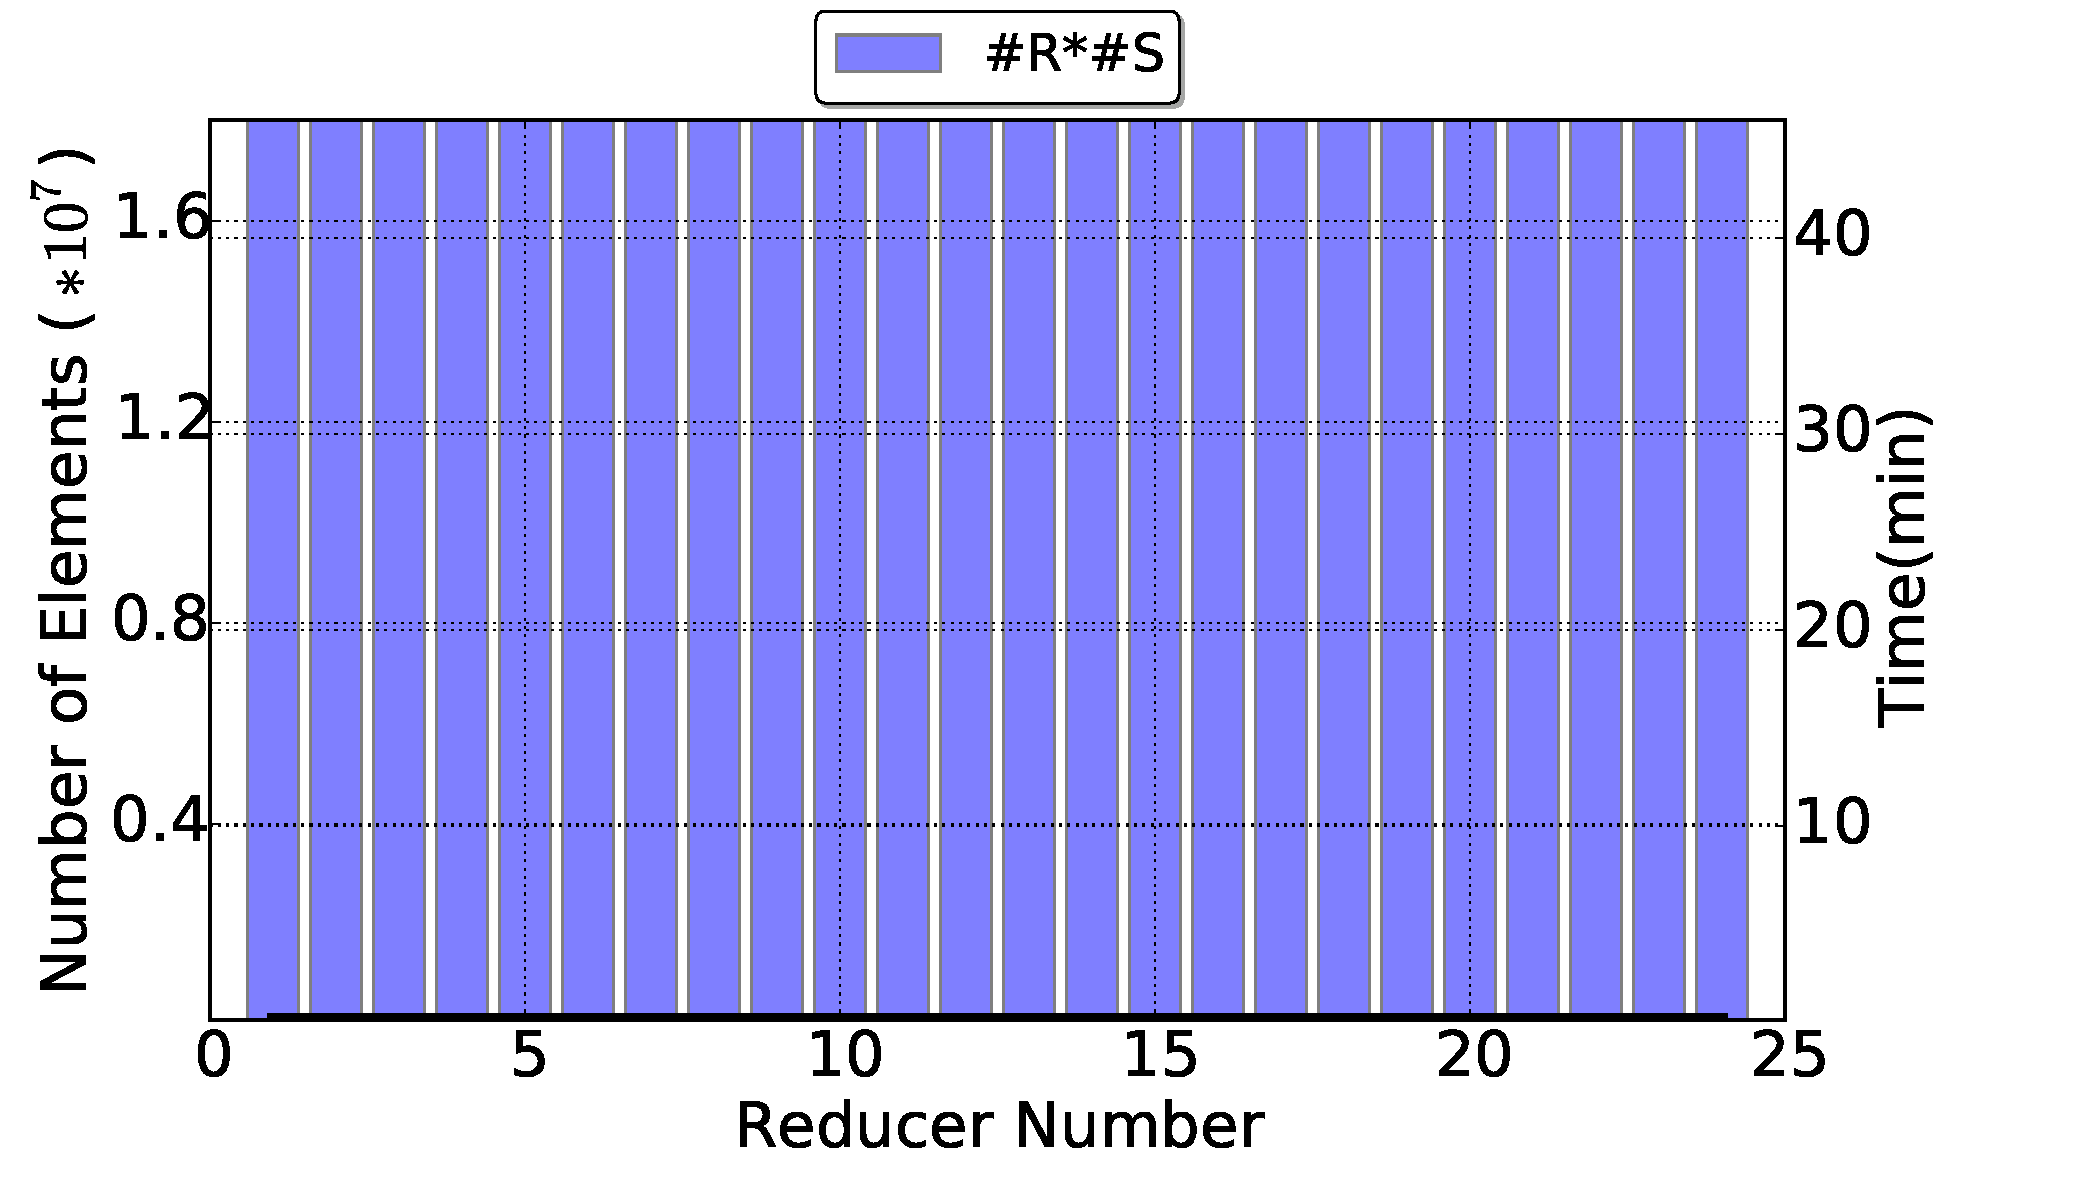
\includegraphics[width=\textwidth]{img-perf/perso/loadbalancing/lsh.pdf}
%                \caption{RankReduce\label{fig:lb_lsh} }
%                
%        \end{subfigure}%
%        \begin{subfigure}[b]{0.3\textwidth}
%                \includegraphics[width=\textwidth]{img-perf/perso/loadbalancing/hzknnj.pdf}
%                \caption{H-ZKNNJ\label{fig:lb_z}, \TODOREP(c'est du au BTree qui est a l'interieur que meme si on a la meme repartition, on a un temps différents)}
%                
%        \end{subfigure}%
% \caption{Load balancing on phase of computing candidates KNN , with Geo dataset, 100000 records, \TODOREP(mm parametrre que geo)}
% \label{fig:load_balancing}\TODO{where do we use b and c?}
%\end{figure*}
%
%
%
%%Voronoi
%\begin{figure*}[h]
%\centering
%%		\begin{subfigure}[b]{0.3\textwidth}
%%                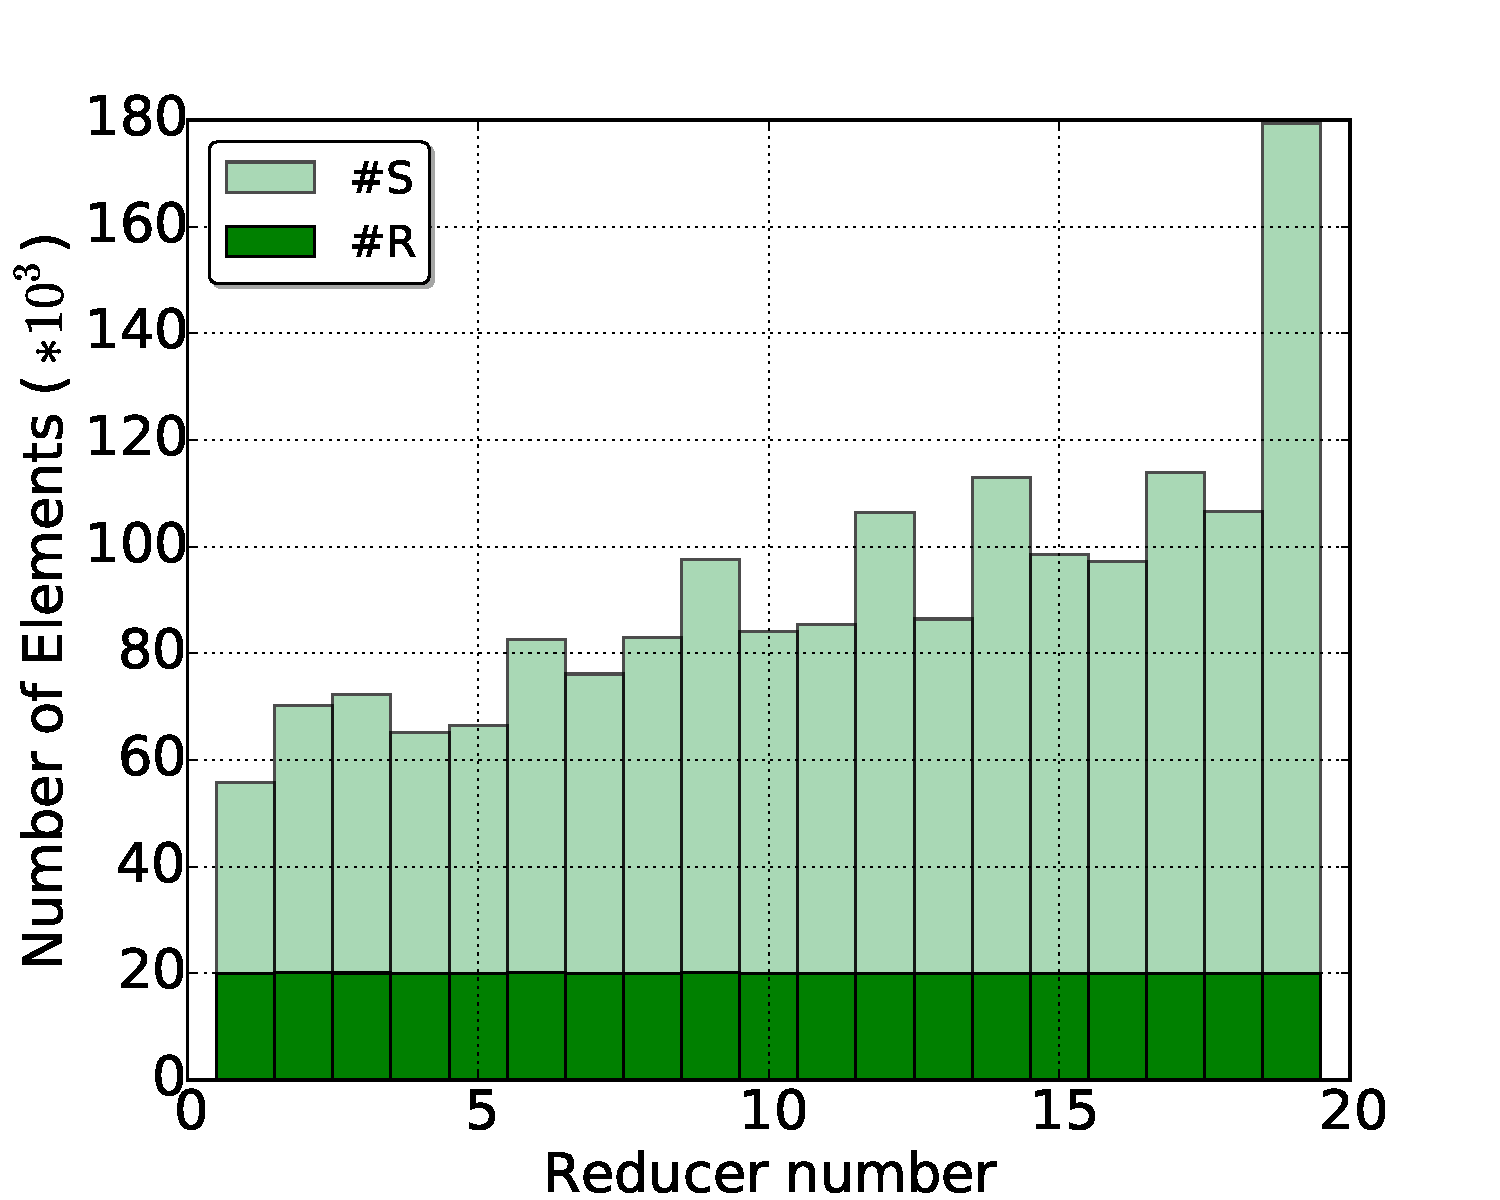
\includegraphics[width=\textwidth]{img-perf/perso/pgbj/geo_20r_400.pdf}
%%                \caption{Geo with 20 reducers\label{fig:geo_20r}}
%%                
%%        \end{subfigure}%
%%        \begin{subfigure}[b]{0.3\textwidth}
%%                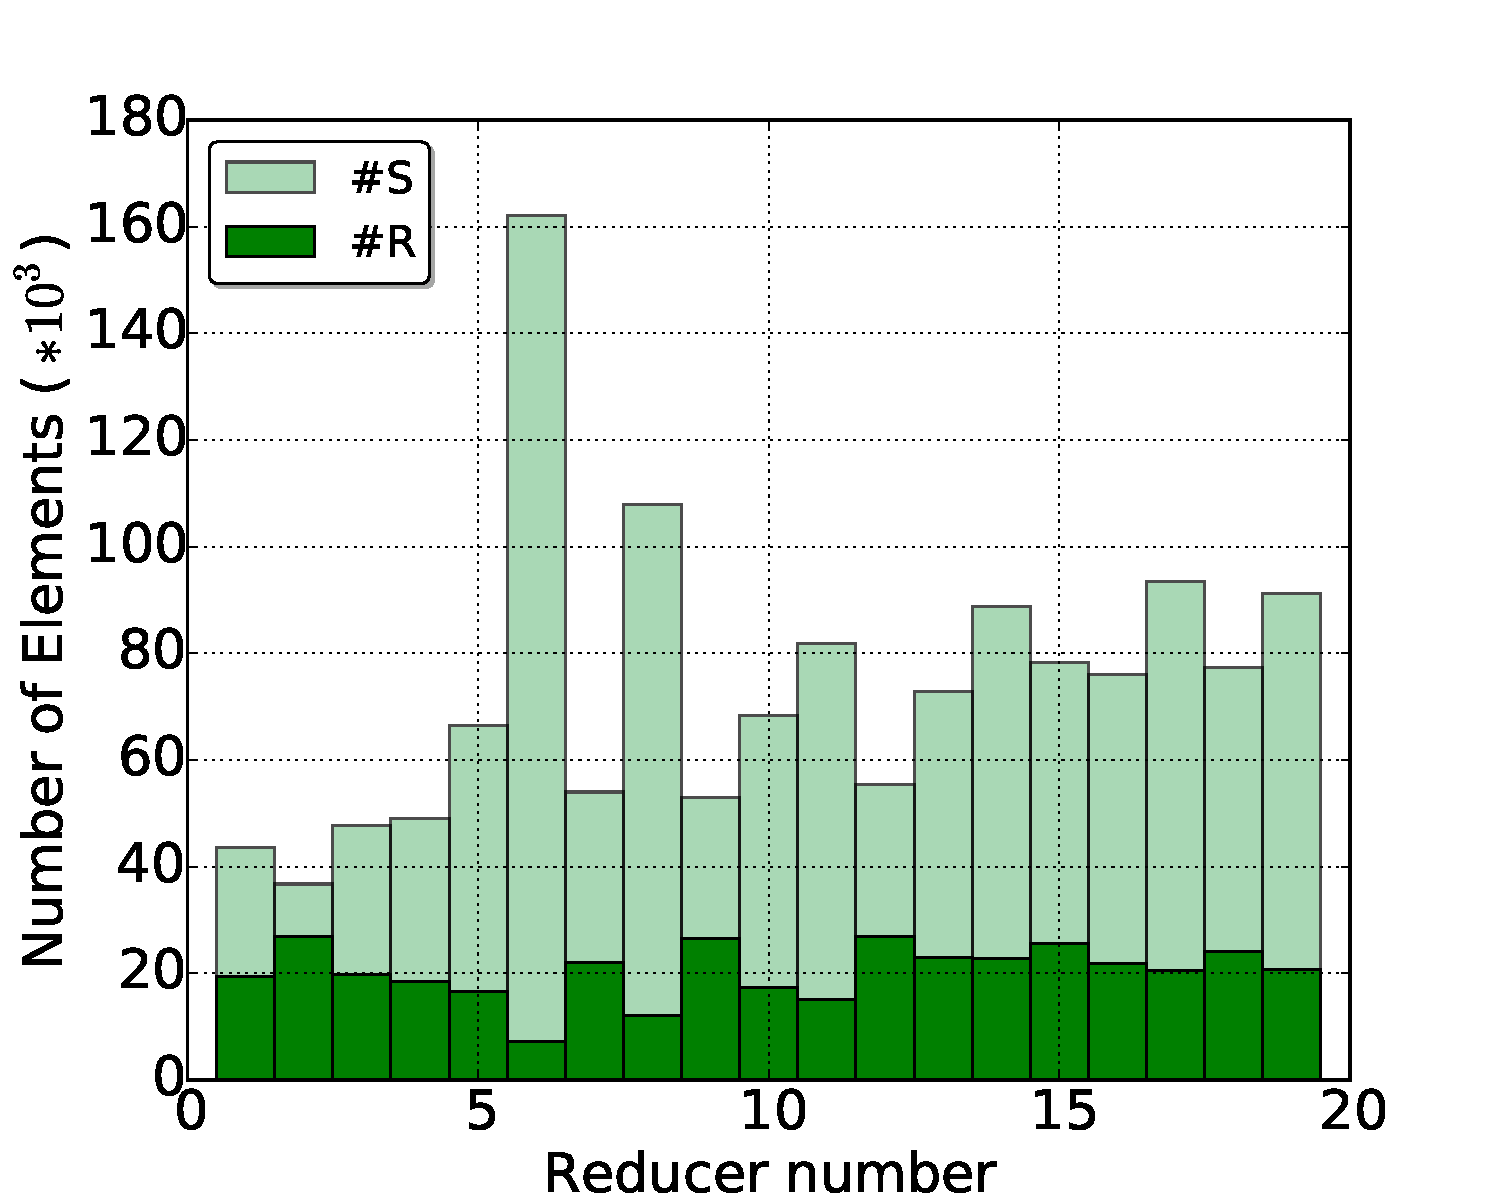
\includegraphics[width=\textwidth]{img-perf/perso/pgbj/greedy_20r_400.pdf}
%%                \caption{Greedy with 20 reducers\label{fig:greedy_20r}}
%%                
%%        \end{subfigure}%
%        \begin{subfigure}[b]{0.3\textwidth}
%                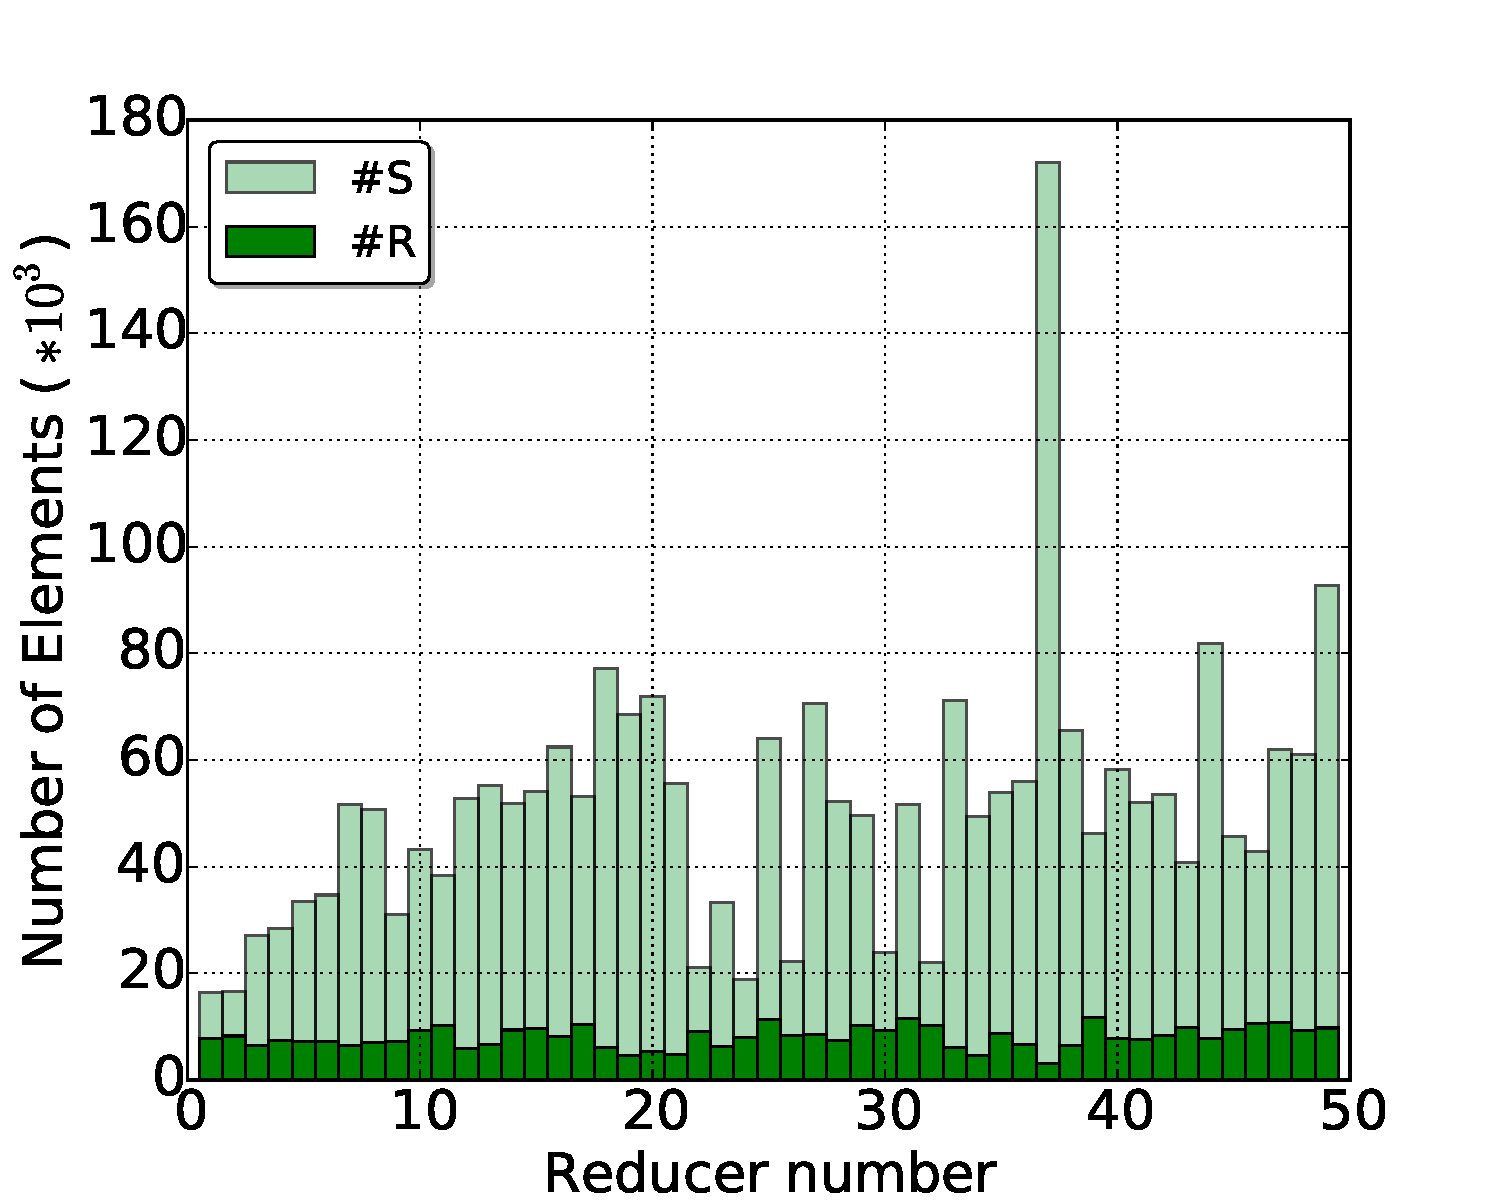
\includegraphics[width=\textwidth]{img-perf/perso/pgbj/greedy_50r_400.pdf}
%                \caption{Greedy with 50 reducers\label{fig:greedy_50r}}
%                
%        \end{subfigure}%
% \caption{Load balancing on phase of computing candidates KNN of different strategies for PGBJ,  Geo dataset , 400000, 3000 pivots, KMeans Sampling, 20 nodes\TODOREP{(temps en secondes !) et pas oblige de mettre vu qu il y en a deja un qui le décrit } } \TODO{Where do we cite this figure?}
% \label{fig:voronoi_lb_exp}
%\end{figure*}
